\documentclass[12pt, a4paper]{report}

\usepackage{libertine}
\usepackage{libertinust1math}
\usepackage{inconsolata}
\usepackage{amsthm, amsmath}
\usepackage[style=german]{csquotes}
\usepackage[pagestyles]{titlesec}
\usepackage[romanian]{babel}
\usepackage{tikz}
\usetikzlibrary{er,positioning}
\usepackage{soul}
\usepackage{tocloft}
\usepackage{enumerate}
\usepackage{setspace}
\usepackage{subcaption}
\usepackage{bm}
\usepackage{xcolor}
\usepackage{todonotes}
\usepackage{graphicx}
\usepackage{array}
\usepackage[all]{xy}
\setcounter{MaxMatrixCols}{20}
\usepackage{fancyhdr}
% \usepackage{natbib}     % citekey hyphenation
\usepackage{marginnote}
\usepackage{imakeidx}
\makeindex[options= -s indices-alph.ist]
\usepackage{hyperref}
\hypersetup{citecolor=blue}
\usepackage{fontawesome}

\newcommand\NN{\mathbb{N}}
\newcommand\ZZ{\mathbb{Z}}
\newcommand\QQ{\mathbb{Q}}
\newcommand\RR{\mathbb{R}}
\newcommand\CC{\mathbb{C}}
\newcommand\AF{\mathbb{A}}
\newcommand\PP{\mathbb{P}}
\newcommand\FF{\mathbb{F}}
\newcommand\bb{\mathbb}
\newcommand\dr{\mathrm}
\newcommand\kal{\mathscr}
\newcommand\fk{\mathfrak}
\newcommand\op{\oplus}
\newcommand\ot{\otimes}
\newcommand\ds{\displaystyle}
\newcommand\id{\indent}
\newcommand\nid{\noindent}
\newcommand\seq{\subseteq}
\newcommand\sneq{\subsetneq}
\newcommand\speq{\supseteq}
\newcommand\spneq{\supsetneq}
\newcommand\rar{\rightarrow}
\newcommand\Rar{\Rightarrow}
\newcommand\xrar{\xrightarrow}
\newcommand\lar{\leftarrow}
\newcommand\Lar{\Leftarrow}
\newcommand\xlar{\xleftarrow}
\newcommand\lrar{\leftrightarrow}
\newcommand\Lrar{\Leftrightarrow}
\newcommand\ideal{\trianglelefteq}
\newcommand\such{\text{ s.t. }}
\newcommand\sk{(\textit{Sketch}) }
\newcommand\rhup{\rightharpoonup}
\newcommand\rhdn{\rightharpoondown}
\newcommand\lhup{\leftharpoonup}
\newcommand\lhdn{\leftharpoondown}
\newcommand\incl{\hookrightarrow}
\newcommand\vid{\emptyset}
\newcommand\wt{\widetilde}
\newcommand\wh{\widehat}
\newcommand\ol{\overline}
\newcommand\Lor{\Longrightarrow}
\newcommand\Lol{\Longleftarrow}
\newcommand\Lolr{\Longleftrightarrow}
\newcommand\ld{{}^\ast}
\newcommand\lgr{{}^{\ast-\text{gr}}}
\newcommand\kap{\Bbbk^a[\kal{P}]}
\newcommand\kcp{\Bbbk^c[\kal{P}]}
\newcommand\fc{\mathfrak{c}}
\newcommand\qq{\enquote}
\newcommand\coli{\protect\varinjlim}
\newcommand\li{\protect\varprojlim}
\newcommand\injr{\rightarrowtail}
\newcommand\surjr{\twoheadrightarrow}
\newcommand\injl{\leftarrowtail}
\newcommand\surjl{\twoheadleftarrow}
\newcommand\sqsb{\sqsubseteq}
% THEOREMS
\newtheoremstyle{dotless}{}{}{\itshape}{}{\bfseries}{:}{ }{}
\theoremstyle{dotless}
\newtheorem{theorem}{Teorem\u{a}}[section]
\newtheorem{proposition}{Propozi\c{t}ie}[section]
\newtheorem{lemma}{Lem\u{a}}[section]
\newtheorem{corollary}{Corola}[section]
\newtheorem{axiom}{Axiom\u{a}}[section]
\newtheorem{principle}{Principiu}[section]
\newtheorem{reg}{Regul\u{a}}[section]
\renewcommand*{\proofname}{Dem.:}

\newtheoremstyle{dotlessdr}{}{}{}{}{\bfseries}{:}{ }{}
\theoremstyle{dotlessdr}
\newtheorem{example}{Exemplu}[section]
\newtheorem{definition}{Defini\c{t}ie}[section]
\newtheorem{remark}{Observa\c{t}ie}[section]
\newtheorem{exercise}{Exerci\c{t}iu}[section]
\numberwithin{equation}{section}
% FONTS
\usepackage[mathscr]{euscript}
\usepackage[normalem]{ulem}
\usepackage{eurosym}
\usepackage{sectsty}
\allsectionsfont{\rmfamily}
\usepackage{anyfontsize}

% PAGE SETUP
\usepackage[portrait]{geometry}
\geometry{
  a4paper,
  left=20mm,
  right=25mm,
  % marginparwidth=40mm,
}
\usepackage{afterpage}
\newcommand\blankpage{
  \null
  \thispagestyle{empty}
  \addtocounter{page}{-1}
  \newpage}
\newenvironment{myenv}[1]
  {\begin{spacing}{#1}}
    {\end{spacing}}

% FANCY SETUP
\usepackage[Glenn]{fncychap}
\usepackage{fancyhdr}
\addto\captionsromanian{\renewcommand{\chaptername}{Secțiunea}}


\begin{document}

\thispagestyle{empty}
\pagestyle{plain} % fix for page numbers

\title{\huge\textbf{Curbe eliptice peste corpuri finite}}
\vspace{1cm}
\author{\Large\textsc{Adrian Manea}}

\maketitle

\pagenumbering{gobble}
\tableofcontents

\setcounter{page}{1} % page 1 after TOC

%%%%%%%%%%%%%%%%%%%%%%%%%%%%%%%%%%%%%%%%%%%%%%%%%%
% MAIN CONTENT
\pagenumbering{arabic}
\pagestyle{fancy}
\fancyhf{}
\rhead{\footnotesize{\color{gray}Curbe eliptice peste corpuri finite}}
\lhead{\footnotesize{\color{gray}Adrian Manea, 510 SLA}}

\pagestyle{plain} % restore page numbering

% DE ADĂUGAT
\addcontentsline{toc}{chapter}{\protect\numberline{}DE ADĂUGAT/CLARIFICAT}
\listoftodos[DE ADĂUGAT/CLARIFICAT]

% CHAPTERS
% ! TEX root = ../curbe.tex

\chapter{Preliminarii}

\section{Varietăți algebrice}

Începem prezentarea cu cîteva preliminarii privitoare la varietăți algebrice
și alte noțiuni elementare de algebră comutativă.

Vom folosi următoarele notații și obiecte:
\begin{itemize}
\item $ K $ este un corp perfect, i.e.\ unul pentru care orice extindere algebrică
  este separabilă;
\item $ \overline{K} $ este o închidere algebrică fixată a lui $ K $;
\item $ \dr{Gal}(\overline{K}/K) = G_{\overline{K}/K} $ este grupul Galois
  al extinderii $ K \seq \overline{K} $.
\end{itemize}

În majoritatea exemplelor, $ K $ va fi (o extindere algebrică a lui) $ \QQ $,
$ \QQ $ sau $ \mathbb{F}_p $.

\begin{definition}\label{def:spatiu-afin}
  \index{spațiu!afin}
  \index{spațiul!punctelor raționale}
  \emph{Spațiul afin} peste corpul $ K $ este mulțimea de $ n $-tupluri:
  \[
    \mathbb{A}^n = \mathbb{A}^n(K) = \{ P = (x_1, \dots, x_n) \in \overline{K}^n \}.
  \]
  Similar, se definește \emph{spațiul punctelor $ K $-raționale} din $ \mathbb{A}^n $,
  care conține restricția $ P \in K^n $.
\end{definition}

Fie $ \overline{K}[X] = \overline{K}[X_1, \dots, X_n] $ un inel de polinoame în $ n $
nedeterminate și fie $ I \ideal \overline{K}[X] $ un ideal. Putem asocia fiecărui
astfel de ideal o submulțime a lui $ \AF^n $:
\[
  V_I = \{ P \in \AF^n \mid f(P) = 0, \quad \forall f \in I \}.
\]

\begin{definition}\label{def:multime-algebrica-afina}
  \index{mulțime!algebrică afină}
  O \emph{mulțime algebrică afină} este o mulțime de forma $ V_I $ ca mai sus.

  Dacă $ V $ este o astfel de mulțime, \emph{idealul} lui $ V $ este:
  \[
    I(V) = \{ f \in \overline{K}[X] \mid f(P) = 0, \quad \forall P \in V \}.
  \]
\end{definition}

Spunem că o mulțime algebrică este \emph{definită} peste $ K $ dacă idealul său
$ I(V) $ poate fi generat de polinoame din $ K[X] $ și notăm aceasta cu $ V/K $.
\index{mulțime!algebrică definită}

Dacă $ V $ este definită peste $ K $, \emph{mulțimea punctelor $ K $-raționale} ale
lui $ V $ este mulțimea:
\[
  V(K) = V \cap \AF^n(K).
\]

\begin{remark}\label{rk:kx-finit-gen}
  Conform teoremei bazei a lui Hilbert, idealele lui $ \overline{K}[X] $ și
  $ K[X] $ sînt finit generate.
\end{remark}

Fie $ V $ o mulțime algebrică și considerăm idealul:
\[
  I(V/K) = \{ f \in K[X] \mid f(P) = 0, \quad \forall P \in V \} = I(V) \cap K[X].
\]

Se poate observa că $ V $ este definită peste $ K $ dacă și numai dacă are loc
relația:
\[
  I(V) = I(V/K) \cdot \overline{K}[X].
\]

Presupunem acum că $ V $ este definită peste $ K $ și fie $ f_1, \dots, f_m \in K[X] $,
generatori ai idealului $ I(V/K) $. Rezultă că $ V(K) $ este mulțimea soluțiilor
$ x = (x_1, \dots, x_n) $ pentru ecuațiile polinomiale:
\[
  f_1(x) = \dots = f_m(x) = 0, \quad x_1, \dots, x_n \in K.
\]

\begin{example}\label{exm:multime-alg1}
  Fie $ V $ mulțimea algebrică din $ \AF^2 $ dată de ecuația $ X^2 - Y^2 = 1 $.

  Atunci $ V $ este definită peste orice corp $ K $.

  Presupunem acum $ \dr{char}K \neq 2 $. Rezultă $ V(K) \simeq \AF^1(K) - \{ 0 \} $,
  o bijecție fiind, de exemplu:
  \begin{align*}
    \AF^1(K) - \{ 0 \} &\to V(K) \\
    t &\mapsto \left( \dfrac{t^2 + 1}{2t}, \dfrac{t^2 - 1}{2t} \right).
  \end{align*}
\end{example}

\begin{example}\label{exm:multime-alg2}
  Mulțimea algebrică $ V : X^n + Y^n = 1 $ este definită peste $ \QQ $ și,
  folosind Marea Teoremă a lui Fermat, pentru orice $ n \geq 3 $, are loc:
  \[
    V(\QQ) = %
    \begin{cases}
      \{(1, 0), (0, 1) \}, & n \text{ impar} \\
      \{(\pm 1, 0), (0, \pm 1)\}, & n \text{ par}
    \end{cases}.
  \]
\end{example}

\begin{example}\label{exm:multime-alg3}
  Mulțimea algebrică $ V: X^2 = Y^3 + 17 $ are multe puncte $ \QQ $-raționale.
  De fapt, se poate arăta că $ V(\QQ) $ este infinită. Cîteva exemple sînt:
  \[
    V(\QQ) = \{ (3, -2), (378661, 5234), \left( \dfrac{2651}{512}, \dfrac{137}{64} \right) \}.
  \]
\end{example}

\begin{definition}\label{def:varietate-afina}
  \index{varietate!afină}
  O mulțime algebrică (afină) se numește \emph{varietate algebrică (afină)} dacă $ I(V) $ este
  un ideal prim al lui $ \overline{K}[X] $.
\end{definition}

Remarcăm că dacă $ V $ este definită peste $ K $, atunci este suficient să verificăm dacă
$ I(V/K) $ este ideal prim al lui $ K[X] $.

Fie $ V/K $ o varietate, adică $ V $ este varietate definită peste $ K $. Atunci
\emph{inelul coordonatelor afine} al $ V/K $ este:
\[
  K[V] = \dfrac{K[X]}{I(V/K)}.
\]

De asemenea, deoarece $ I(V/K) $ este ideal prim, rezultă că $ K[V] $ este
domeniu de integritate. Corpul său de fracții se notează $ K(V) $ și se numește
\emph{corpul de funcții} al lui $ V/K $.

Similar putem formula înlocuind $ K $ cu $ \overline{K} $.

În plus, orice element al $ \overline{K}[V] $ se definește pînă la un element din
$ I(V/\overline{K}) $, deci pînă la un polinom ce se anulează pe $ V $. Rezultă
că $ f \in \overline{K}[V] $ induce o funcție $ f : V \to \overline{K} $.

\begin{definition}\label{def:varietate-alg-dim}\index{varietate!afină!dimensiune}
  Fie $ V $ o varietate algebrică.

  \emph{Dimensiunea} varietății, notată $ \dim V $, este gradul de transcendență
  al extinderii $ \overline{K}(V) $ peste $ \overline{K} $.
\end{definition}

\begin{example}\label{exm:dim}
  $ \dim\AF^n = n $, deoarece $ \overline{K}(\AF^n) = \overline{K}(X_1, \dots, X_n) $.

  Dacă $ V \seq \AF^n $ este dat de o ecuație polinomială neconstantă $ f(X_1, \dots, X_n) = 0 $,
  atunci $ \dim V = n - 1 $.
\end{example}

Vom fi interesați de proprietatea de \emph{netezime}, care se definește prin analogul condiției
de existență a planului tangent:

\begin{definition}\label{def:neted}
  \index{varietate!netedă}
  Fie $ V $ o varietate algebrică, $ P \in V, f_1, \dots, f_m \in \overline{K}[X] $ o mulțime
  de generatori pentru $ I(V) $.

  $ V $ se numește \emph{nesingulară (netedă)} în $ P $ dacă matricea jacobiană
  $ \left( \dfrac{\partial f_i}{\partial X_j}(P) \right) $ are rangul $ n - \dim V $.
\end{definition}

\begin{example}\label{exm:dim}
  Fie $ V $ dată de o ecuație polinomială neconstantă $ f(x_1, \dots, x_n) = 0 $.

  Atunci $ \dim V $ = $ n - 1 $, deci $ P $ este singularitate dacă și numai dacă
  $ \dfrac{\partial f}{\partial x_i}(P) = 0, \forall 1 \leq i \leq n $. Totodată,
  $ f(P) = 0 $, deci în total obținem $ n + 1 $ condiții pe $ n $ nedeterminate.
\end{example}

\begin{example}\label{exm:dim2}
  Fie două varietăți:
  \[
    V_1: Y^2 = X^3 + X \quad \text{și} \quad V_2: Y^2 = X^3 + X^2.
  \]

  Punctele lor singulare trebuie să satisfacă:
  \[
    V_1^{\text{sing}}: 3X^2 + 1 = 2Y = 0 \quad \text{și} \quad %
    V_2^{\text{sing}}: 3X^2 + 2X = 2Y = 0.
  \]

  Rezultă că $ V_1 $ nu are singularități, dar $ V_2 $ are, originea $ (0, 0) $.
\end{example}

Putem formula și o altă caracterizare a netezimii, prin funcții definite pe varietate.
Fie $ P $ un punct arbitrar din $ V $. Definim idealul $ M_P \ideal \overline{K}[V] $ prin:
\[
  M_P = \{ f \in \overline{K}[V] \mid f(P) = 0 \}.
\]
Se poate observa că $ M_P $ este maximal, deoarece avem izomorfismul:
\begin{align*}
  \overline{K}[V]/M_P &\to \overline{K} \\
  f &\mapsto f(P).
\end{align*}

Rezultă că grupul factor $ M_P/M_P^2 $ este un $ \overline{K} $-spațiu vectorial
finit dimensional.

Are loc:
\begin{proposition}\label{pr:var-alg}
  Fie $ V $ o varietate algebrică.

  Punctul $ P \in V $ este nesingular dacă și numai dacă $ \dim_{\overline{K}} M_P/M_P^2 = \dim V $.
\end{proposition}

\begin{example}\label{exm:nesing}
  Reluăm cazul anterior al varietăților $ V_1 $ și $ V_2 $ (exemplul \ref{exm:dim2}) și
  fie $ P = (0, 0) $.

  În ambele cazuri, $ M_P $ este generat de $ X $ și $ Y $, deci $ M_P^2 $ este generat de
  $ X^2, XY $ și $ Y^2 $.

  Pentru $ V_1 $ avem:
  \[
    X = Y^2 - X^3 \equiv 0 \text{ mod } M_P^2,
  \]
  deci $ M_P^2 $ este generat doar de $ Y $.

  Dar pentru $ V_2 $ nu avem nicio relație netrivială între $ X $ și $ Y $ modulo $ M_P^2 $, deci
  ambele nedeterminate sînt necesare ca generatori.

  Rezultă că $ V_1 $ e netedă, dar $ V_2 $ nu este, deoarece $ \dim V_{1,2} = 1 $.
\end{example}

Folosind idealul maximal, avem:
\begin{definition}\label{def:inel-local}
  \emph{Inelul local} al varietății $ V $ în $ P $, notat $ \overline{K}[V]_P $, este localizatul
  în $ M_P $, adică:
  \[
    \overline{K}[V]_P = \{ F \in \overline{K}(V) \mid F = f/g, \quad f,g \in \overline{K}[V], g(P) \neq 0 \}.
  \]
\end{definition}

Remarcăm că din $ F = f/g $ rezultă că $ F(P) = f(P)/g(P) $ este corect definită.

Funcțiile din $ \overline{K}[V]_P $ se numesc \emph{regulate} (sau \emph{definite}) în $ P $.

%%%%%%%%%%%%%%%%%%%%%%%%%%%%%%%%%%%%%%%%%%%%%%%%%%%%%%%%%%%%%%%%%%%%%%

\section{Varietăți proiective}

Definim varietățile proiective ca fiind colecția de linii ce trec prin originea
unui spațiu afin de dimensiune imediat superioară.

\begin{definition}\label{def:spatiu-proiectiv}
  \index{spațiu!proiectiv}
  \emph{Spațiul $ n $-proiectiv} peste $ K $, notat $ \PP^n $ sau $ \PP^n(\overline{K}) $,
  este mulțimea tuturor $ (n + 1) $-tuplurilor $ (x_0, \dots, x_n) \in \AF^{n + 1} $,
  astfel încît cel puțin o coordonată $ x_i $ este nenulă modulo echivalența:
  \[
    (x_0, \dots, x_n) \sim (y_0, \dots, y_n) \Leftrightarrow \exists \lambda %
    \in \overline{K}^\times \text{ a.\^{i}. } x_i = \lambda y_i, \forall i.
  \]

  Clasa de echivalență
  $ \{(\lambda x_0, \dots, \lambda x_n) \mid \lambda \in \overline{K}^\times \} $
  se notează $ [x_0, \dots, x_n] $, iar $ x_0, \dots, x_n $ se numesc \emph{coordonatele %
  omogene} ale punctului respectiv în $ \PP^n $.
\end{definition}

De asemenea, mulțimea punctelor $ K $-raționale din $ \PP^n $ este:
\[
  \PP^n(K) = \{ [x_0, \dots, x_n] \in \PP^n \mid x_i \in K \}.
\]

\begin{remark}\label{rk:proj}
  Pentru $ P = [x_0, \dots, x_n] \in \PP^n(K) $, \emph{nu} rezultă că fiecare $ x_i \in K $.
  În schimb, alegem un $ i $ cu $ x_i \neq 0 $ și rezultă că $ x_j / x_i \in K $, pentru
  orice $ j $.
\end{remark}

\begin{definition}\label{def:corp-minimal}
  \index{corp!minimal}
  Fie $ P = [ x_0, \dots, x_n ] \in \PP^n(\overline{K}) $. \emph{Corpul minimal de definiție}
  pentru $ P $ peste $ K $ este corpul:
  \[
    K(P) = K(x_0/x_i, \dots, x_n/x_i), \quad \forall i, \text{ cu } x_i \neq 0.
  \]
\end{definition}

\begin{definition}\label{def:polinom-omogen}
  \index{polinom!omogen}
  Un polinom $ f \in \overline{K}[X] $ se numește \emph{omogen de grad $ d $} dacă:
  \[
    f(\lambda x_0, \dots, \lambda x_n) = \lambda^d f(x_0, \dots, x_n), %
    \quad \forall \lambda \in \overline{K}.
  \]

  Un \emph{ideal omogen} al lui $ \overline{K}[X] $ este generat de polinoame omogene.
\end{definition}

Fiecărui ideal omogen îi putem asocia o submulțime a $ \PP^n $:
\[
  V_I = \{ P \in \PP^n \mid f(P) = 0, \text{ pentru orice } f \in I \text{ omogen } \}.
\]

\begin{definition}\label{def:multime-proiectiva}
  \index{mulțime!proiectivă}
  O \emph{mulțime (algebrică) proiectivă} este una de forma $ V_I $ ca mai sus.

  Idealul omogen al unei mulțimi proiective, notat $ I(V) $, este idealul lui
  $ \overline{K}[X] $ generat de:
  \[
    \{ f \in \overline{K}[X] \mid f \text{ omogen }, f(P) = 0, \forall P \in V \}.
  \]
\end{definition}

Similar putem descrie și $ V/K $ și $ V(K) = V \cap \PP^n(K) $.

\begin{example}\label{exm:dreapta-proj}
  O \emph{dreaptă} în $ \PP^2 $ este o mulțime algebrică dată de
  $ aX + bY + cZ = 0 $, cu $ a, b, c \in \overline{K} $, nu toate nule.

  Dacă, de exemplu, $ c \neq 0 $, atunci dreapta este definită peste orice corp
  care conține $ a/c $ și $ b/c $.

  În general, un \emph{hiperplan} în $ \PP^n $ este dat de o ecuație:
  \[
    a_0 X_0 + a_1 X_1 + \dots + a_n X_n = 0, %
    \quad a_i \in \overline{K}, \text{ nu toate nule}.
  \]
\end{example}

\begin{example}\label{exm:var-proj}
  Fie $ V $ în $ \PP^2 $ dată de $ X^2 + Y^2 = Z^2 $.

  Atunci, pentru orice corp $ K $, cu $ \dr{char}K \neq 2 $, avem $ V(K) \simeq \PP^1(K) $,
  de exemplu prin:
  \begin{align*}
    \PP^1(K) &\to V(K) \\
    [s, t] &\mapsto [s^2 - t^2, 2st, s^2 + t^2].
  \end{align*}
\end{example}

%%%%%%%%%%%%%%%%%%%%%%%%%%%%%%%%%%%%%%%%%%%%%%%%%%%%%%%%%%%%%%%%%%%%%%
\subsection{Aplicație aritmetică}

Fie un punct din $ \PP^n(\QQ) $, de coordonate $ [x_0, \dots, x_n], x_i \in \QQ $.

Putem presupune că am înmulțit cu numitorul comun și am eliminat factorii comuni,
deci putem presupune $ x_i \in \ZZ, \dr{gcd}(x_i) = 1 $. Rezultă că punctul
$ P $ determină coordonatele omogene $ x_i $, \emph{pînă la un semn}.

În general, dacă un ideal al unei mulțimi algebrice definite peste $ \QQ $,
$ V / \QQ $, este generat de polinoame omogene $ f_1, \dots, f_m \in \QQ[X] $,
descrierea $ V(\QQ) $ revine la a rezolva ecuațiile omogene:
\[
  f_1(x_0, \dots, x_n) = \dots = f_m(x_0, \dots, x_n) = 0, \quad \dr{gcd}(x_i) = 1.
\]

\begin{example}\label{exm:proj-aritm}
  Fie $ V : X^2 + Y^2 = 3Z^2 $, definit peste $ \QQ $, dar $ V(\QQ) = \emptyset $.
  Într-adevăr, presupunem că $ [x, y, z] \in V(\QQ) $, cu $ x, y, z \in \ZZ $ și
  $ \dr{gcd}(x, y, z) = 1 $. Rezultă $ x^2 + y^2 \equiv 0 \text{ mod } 3 $,
  dar cum $ -1 $ nu este pătrat modulo 3, rezultă că $ x \equiv y \equiv 0 $
  modulo 3, deci $ x^2, y^2 \vdots 3^2 $, adică $ 3 \mid z $, contradicție
  cu $ \dr{gcd}(x, y, z) = 1 $.
\end{example}

Așadar, ideea generală este că, pentru a arăta că $ V(\QQ) = \emptyset $, este
suficient să arătăm că ecuațiile omogene corespunzătoare nu au soluții nenule
\emph{modulo $ p $}, pentru orice prim $ p $ (sau pentru orice putere a unui prim).

Spus mai simplu, avem implicația $ V(\QQ) = \emptyset \Rightarrow V(\QQ_p) = \emptyset $,
pentru orice corp p-adic $ \QQ_p $. Mai departe, implicația poate continua cu $ V(\RR) = \emptyset $.

Însă \emph{reciproca este falsă!} Se poate arăta că, pentru varietatea:
\[
  V: 3X^2 + 4Y^2 + 5Z^3 = 0,
\]
avem $ V(\QQ_p) \neq \emptyset, \forall p $, dar $ V(\QQ) = \emptyset $.

\begin{definition}\label{def:var-proj}
  \index{varietate!proiectivă}
  O mulțime algebrică proiectivă se numește \emph{varietate proiectivă} dacă
  idealul omogen $ I(V) $ este prim în $ \overline{K}[X] $.
\end{definition}

Fie $ f(Y) \in \overline{K}[Y] $. Definim:
\[
  f^\ast(x_0, \dots, x_n) = x_i^d f \left(\dfrac{x_0}{x_i}, \dfrac{x_1}{x_i}, \dots, %
    \dfrac{x_{i - 1}}{x_i}, \dfrac{x_{i + 1}}{x_i}, \dots, \dfrac{x_n}{x_i} \right),
\]
unde $ d = \dr{deg}f $ este cel mai mic întreg care face $ f^\ast $ polinom.

Spunem că $ f^\ast $ este \emph{omogenizatul} lui $ f $ în raport cu $ x_i $.
\index{polinom!omogenizat}

\begin{definition}\label{def:inchidere-proi}
  \index{varietate!proiectivă!închidere proiectivă}
  Fie $ V \seq \AF^n $ o mulțime algebrică afină, cu idealul $ I(V) $ și
  fie $ V $ o submulțime a $ \PP^n $ prin:
  \begin{align*}
    V \seq \AF^n &\xrar{\phi_i} \PP^n \\
    \phi_i(y_1, \dots, y_n) &\mapsto [y_1, \dots, y_{i-1}, 1, y_i, \dots, y_n].
  \end{align*}

  \emph{Închiderea proiectivă} a lui $ V $, notată $ \overline{V} $, este
  mulțimea proiectivă al cărui ideal omogen $ I(\overline{V}) $ este generat
  de omogenizatele generatorilor lui $ I(V) $.

  Punctele din $ V - \overline{V} $ se numesc \emph{puncte la infinit} din $ V $.
\end{definition}

\begin{example}\label{exm:punct-infinit}
  Fie $ V $ proiectivă, definită de $ Y^2 = X^3 + 17 $.

  Rezultă că $ V $ este dată în $ \PP^2 $ de:
  \[
    \overline{Y}^2 \overline{Z} = \overline{X}^3 + 17 \overline{Z}^3, \quad %
    X = \overline{X}/\overline{Z}, Y = \overline{Y}/\overline{Z}.
  \]

  Varietatea are un singur punct la infinit, $ [0, 1, 0] $, obținut din
  $ \overline{Z} = 0 $. Rezultă:
  \[
    V(\QQ) = \{ (x, y) \in \AF^2(\QQ) \mid y^2 = x^3 + 17 \} \cup \{ [0, 1, 0] \}.
  \]
\end{example}

\begin{definition}\label{def:corp-functii}
  Fie $ V/K $ o varietate proiectivă și fie $ \AF^n \seq \PP^n $ astfel încît
  $ V \cap \AF^n \neq \emptyset $. Atunci se definește:
  \[
    \dim V = \dim (V \cap \AF^n).
  \]

  \emph{Corpul de funcții} $ K(V) $ este corpul de funcții al $ V \cap \AF^n $.
\end{definition}

\begin{remark}\label{rk:alegeri}
  Pentru alegeri diferite ale lui $ \AF^n $, obținem izomorfisme canonice între
  rezultate.
\end{remark}

Similar, \emph{netezimea} în varietăți proiective $ V $ se traduce în $ V \cap \AF^n $.

%%% Local Variables:
%%% mode: latex
%%% TeX-master: "../curbe"
%%% End:

% ! TEX root = ../curbe.tex
\chapter{Curbe algebrice}

Printr-o \emph{curbă algebrică} vom înțelege o varietate proiectivă de
dimensiune 1. Vom lucra, în general, cu curbe netede.

Notațiile specifice sînt:
\begin{itemize}
\item $ C/K $: curba $ C $ este definită peste corpul $ K $;
\item $ \overline{K}(C) $: corpul de funcții al lui $ C $ peste $ K $;
\item $ \overline{K}[C]_P $: inelul local al lui $ C $ în punctul $ P $;
\item $ M_P $: idealul maximal al inelului local $ \overline{K}[C]_P $.
\end{itemize}

\begin{definition}\label{def:valuare-norm}
  \index{valuare!normalizată}
  \index{uniformizator}
  Fie $ C $ o curbă și $ P \in C $ un punct neted.

  \emph{Valuarea normalizată} pe $ \overline{K}[C]_P $ este dată de:
  \begin{align*}
    \dr{ord}_P : \overline{K}[C]_P &\to \NN \cup \{ \infty \} \\
    \dr{ord}_P(f) &= \sup \{ d \in \ZZ \mid f \in M_P^d \}.
  \end{align*}

  Folosind $ \dr{ord}_P(f/g) = \dr{ord}_P(f) - \dr{ord}_P(g) $, putem
  extinde valuarea la $ \ZZ $.

  Un \emph{uniformizator} pentru $ C $ în $ P $ este orice funcție
  $ t \in \overline{K}(C) $, cu $ \dr{ord}_P t = 1 $, adică
  $ t $ este generator pentru dealul $ M_P $.
\end{definition}

Pentru $ C $ și $ P $ ca mai sus, fie $ f \in \overline{K}(C) $.
Se definește \emph{ordinul} lui $ f $ în $ P $ prin $ \dr{ord}_P f $.
Dacă ordinul este pozitiv, spunem că $ f $ are zero în $ P $; altfel,
$ f $ are singularitate (pol) în $ P $. Dacă ordinul este pozitiv,
spunem că $ C $ este \emph{definită} în $ P $ și putem calcula $ f(P) $.
Altfel, $ f(P) = \infty $.

\begin{example}\label{exm:ordin}
  Reluăm unul dintre exemplele anterioare (exemplul \ref{exm:dim2}):
  \[
    C_1: Y^2 = X^3 + X, \quad C_2: Y^2 = X^3 + X^2.
  \]
  Ambele curbe au cîte o singularitate la infinit. Fie $ P = (0, 0) $.
  Atunci $ C_1 $ este netedă în $ P $, dar $ C_2 $ nu este.

  Idealul maximal $ M_P $ al lui $ \overline{K}[C_1]_P $ are proprietatea că
  $ M_P/M_P^2 $ este generat de $ Y $, deci:
  \[
    \dr{ord}_P Y = 1, \quad \dr{ord}_P X = 2, \quad \dr{ord}_P(2Y^2 - X) = 2,
  \]
  ultima egalitate rezultînd din $ 2Y^2 - X = 2X^3 + X $.
\end{example}

%%%%%%%%%%%%%%%%%%%%%%%%%%%%%%%%%%%%%%%%%%%%%%%%%%%%%%%%%%%%%%%%%%%%%%

\section{Divizori}

\begin{definition}\label{def:divizor}
  \index{curbe!divizori}
  Fie $ C $ o curbă algebrică. \emph{Grupul divizorilor} curbei, notat
  $ \dr{Div}C $, este grupul abelian liber ($ \ZZ $-modulul) generat de
  punctele de pe $ C $.

  Deci orice $ D \in \dr{Div}C $ este o sumă formală:
  \[
    D = \sum_{P \in C} n_P(P),
  \]
  unde $ n_P \in \ZZ $ și $ n_P = 0 $ pentru majoritatea $ P \in C $.

  \emph{Gradul divizorului} $ D $ se definește prin:
  \[
    \dr{deg} D = \sum_{P \in C} n_P.
  \]
\end{definition}

%%% Local Variables:
%%% mode: latex
%%% TeX-master: "../curbe"
%%% End:

%! TEX root = ../curbe.tex

\chapter{Curbe eliptice}

\section{Ecuații Weierstrass}

Vom studia în special curbe eliptice, care sînt curbe de gen 1,
cu un punct-bază specificat. Vom vedea că orice astfel de curbă poate
fi gîndită ca locul geometric în $ \PP^2 $ al unei ecuații cubice cu un punct,
punctul bază, pe linia de la infinit. Apoi, după o schimbare de coordonate,
orice curbă eliptică se poate prezenta sub forma:
\[
      Y^2Z + a_1 XYZ + a_3 YZ^2 = X^3 + a_2X^2Z + a_4XZ^2 + a_6Z^3.
\]
În acest caz, punctul bază este $ O = [0, 1, 0] $, iar $ a_i \in \overline{K} $.

Studiem acum curbele eliptice care sînt date cu formule explicite,
numite \emph{ecuații Weierstrass}.

Pentru simplificarea notației, vom lucra cu coordonatele neomogene,
$ x = X/Z $ și $ y = Y/Z $ și atunci, putem scrie curba:
\[
      E : y^2 + a_1 xy + a_3 y = x^3 + a_2 x^2 + a_4 x + a_6,
\]
ținînd cont și de un punct $ O = [0, 1, 0] $ la infinit. Ca în cazul
oricărei varietăți, dacă $ a_i \in K $, spunem că avem o curbă $ E $
\emph{definită peste $ K $}.

Presupunem că lucrăm cu $ \dr{char}(\overline{K}) \neq 2 $ și atunci
putem simplifica ecuația, cu substituția:
\[
    y \mapsto \dfrac{1}{2} \left( y - a_1x - a_3 \right),
\]
care conduce la ecuația:
\[
      E : y^2 = 4x^3 + b_2 x^2 + 2b_4 x + b_6,
\]
cu notațiile:
\[
      b_2 = a_1^2 + 4a_4, \quad b_4 = 2a_4 + a_1a_3, \quad b_6 = a_3^2 + 4a_6.
\]
Mai definim și:
\begin{align*}
    b_8 &= a_1^2 a_6 + 4a_2a_6 - a_1a_3a_4 + a_2a_3^2 - a_4^2 \\
    c_4 &= b_2^2 - 24b_4 \\
    c_6 &= -b_2^3 + 36b_2b_4 - 216b_6 \\
    \Delta &= -b_2^2b_8 - 8b_4^3 - 27b_6^2 + 9b_2b_4b_6 \\
    j &= c_4^3 / \Delta \\
    \omega &= \dfrac{dx}{2y + a_1x + a_3} = \dfrac{dy}{3x^2 + 2a_2x + a_4 - a_1y}.
\end{align*}

Relațiile simple între aceste cantități sînt:
\[
    4b_8 = b_2b_6 - b_4^2, \quad \text{și} \quad 1728\Delta = c_4^3 - c_6^2.
\]

Mai departe, dacă $ \dr{char}\overline{K} \neq 2, 3 $, putem face substituția:
\[
    (x, y) \mapsto \left( \dfrac{x - 3b_2}{36}, \dfrac{y}{108} \right),
\]
care elimină termenul cu $ x^2 $ și ajungem la:
\[
      E : y^2 = x^3 - 27c_4x - 54c_6.
\]

\begin{definition}\label{def:invarianti-weierstrass}
    \index{invariant Weierstrass!discriminant}
    \index{invariant Weierstrass!j}
    \index{invariant Weierstrass!diferențial}
    Cantitatea $ \Delta $ se numește \emph{discriminantul} ecuației Weierstrass,
    cantitatea $ j $ se cheamă $ j $-invariantul curbei eliptice, iar
    $ \omega $ este \emph{invariantul diferențial} asociat ecuației.
\end{definition}

Considerăm acum o situație generală. Fie $ P = (x_0, y_0) $ un punct arbitrar care
satisface o ecuație de tip Weierstrass:
\[
    f(x, y) = y^2 + a_1 xy + a_3 y - x^3 - a_2x^2 - a_4 x - a_6 = 0
\]
și mai presupunem că $ P $ este o singularitate pentru curba $ f(x, y) = 0 $, deci
\[
    \dfrac{partial f}{\partial x}(P) = \dfrac{\partial f}{\partial y}(P) = 0.
\]
Rezultă că există coeficienți $ \alpha, \beta \in \overline{K} $ astfel încît
dezvoltarea Taylor a polinomului $ f(x, y) $ în jurul lui $ P $ se poate scrie:
\[
    f(x, y) - f(x_0, y_0) = ((y - y_0) - \alpha(x - x_0))((y - y_0) - \beta(x - x_0)) - %
    (x - x_0)^3.
\]

\begin{definition}\label{def:nod}
    Folosind notațiile de mai sus, singularitatea $ P $ se numește \emph{nod} dacă
    $ \alpha \neq \beta $, iar în acest caz, curbele:
    \[
        y - y_0 = \alpha(x - x_0) \quad \text{și} \quad y - y_0 = \beta(x - x_0)
    \]
    se numesc \emph{tangentele în $ P $}. Reciproc, dacă $ \alpha = \beta $,
    spunem că $ P $ este \emph{vîrf} (eng.\ \textit{cusp}), caz în care
    tangenta la $ P $ este dată de:
    \[
        y - y_0 = \alpha(x - x_0).
    \]
\end{definition}

%%%%%%%%%%%%%%%%%%%%%%%%%%%%%%%%%%%%%%%%%%%%%%%%%%%%%%%%%%%%%%%%%%%%%%
\section{Structura de grup}

Fie $ E $ o curbă eliptică dată de o ecuație Weierstrass. Rezultă că
$ E \seq \PP^2 $ conține puncte $ P = (x, y) $ care satisfac ecuația
Weierstrass, împreună cu punctul $ O = [0, 1, 0] $ de la infinit.

Fie $ L \seq \PP^2 $ o dreaptă. Atunci, deoarece ecuația are gradul 3,
dreapta $ L $ intersectează $ E $ în exact 3 puncte, pe care le notăm
$ P, Q, R $.

\begin{definition}\label{def:adunare-eliptic}
    Fie $P, Q \in E $ și fie $ L $ dreapta prin $ P $ și $ Q $ (dacă $ P = Q $,
    atunci $ L $ este tangenta în $ P $). Fie $ R $ un al treilea punct
    de intersecție a lui $ L $ cu $ E $.

    Fie $ L' $ dreapta prin $ R $ și $ O $. Atunci $ L' $ intersectează
    $ E $ în $ R, O $ și un al treilea punct. Acest al treilea punct se notează
    $ P \oplus Q $.
\end{definition}

Operația este ilustrată în figura \ref{fig:adunare-el}.
\begin{figure}[!htbp]
    \centering
    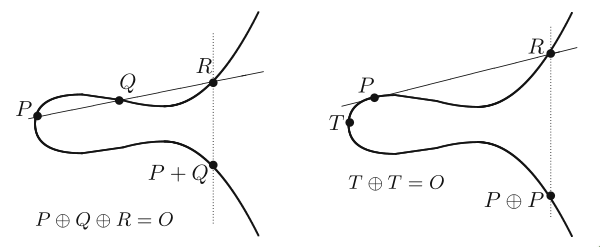
\includegraphics[scale=0.5]{figs/adunare-el.png}
    \caption{\textit{Adunarea punctelor pe o curbă eliptică, \cite{sil09}, p.\ 51}}
    \label{fig:adunare-el}
\end{figure}

Cu acestea, se obține că $ (E, \oplus) $ formează un grup abelian, cu elementul
neutru $ O = [0, 1, 0] $. Pentru simplitate, în continuare vom nota operațiile
cu notațiile obișnuite, $ \oplus \mapsto +, \ominus \mapsto - $.

\begin{example}\label{exm:eliptic-grup}
    Fie curba eliptică $ E/\QQ $:
    \[
          E : y^2 = x^3 + 17.
    \]
    Calcule simple găsesc cîteva puncte cu coordonate întregi:
    \[
        P_1 = (-2, 3), P_2 = (-1, 4), P_3 = (2, 5), P_4 = (4, 9), P_5 = (8, 23).
    \]
    Folosind operația de grup, se pot verifica relațiile:
    \[
          P_5 = -2 \cdot P_1, \quad P_4 = P_1 - P_3.
    \]
    Se poate arăta că orice punct rațional $ P \in E(\QQ) $ poate fi scris sub forma:
    \[
          P = mP_1 + nP_3, \quad m, n \in \ZZ,
    \]
    ceea ce ne arată că $ E(\QQ) \simeq \ZZ \times \ZZ $.
\end{example}>

%%%%%%%%%%%%%%%%%%%%%%%%%%%%%%%%%%%%%%%%%%%%%%%%%%%%%%%%%%%%%%%%%%%%%
\section{Curbe eliptice}

Fie $ E $ o curbă netedă de gen 1.

\begin{definition}\label{def:curba-el}
    O \emph{curbă eliptică} este o pereche $ (E, O) $, alcătuită dintr-o
    curbă nesingulară $ E $ de gen 1 și un punct $ O \in E $.

    Curba se numește \emph{definită peste corpul $ K $}, notat $ E/K $,
    dacă $ E $ este o curbă definită peste $ K $, iar $ O \in E(K) $.
\end{definition}

Relevanța ecuației Weierstrass reiese din:
\begin{proposition}\label{prop:weierstrass-eliptic}
    Fie $ E $ o curbă eliptică definită peste $ K $.
    \begin{enumerate}[(a)]
        \item Există funcțiile $ x, y \in K(E) $ astfel încît aplicația:
            \[
                \phi : E \to \PP^2, \quad \phi = [x, y, 1]
            \]
           dă un izomorfism între $ E/K $ și o curbă dată de o ecuație Weierstrass:
           \[
               C : Y^2 + a_1 XY + a_3 Y = X^3 + a_2 X^2 + a_4 X + a_6,
           \]
           cu coeficienții $ a_1, \dots, a_6 \in K $ și $ \phi(O) = [0, 1, 0] $.

           Funcțiile $ x, y $ se numesc \emph{coordonatele Weierstrass} ale
           curbei eliptice $ E $.
       \item Orice două ecuații Weierstrass pentru curba fixată $ E $ sînt
           legate printr-o schimbare de variabile de forma:
           \[
                 X = u^2 X' + r, \quad Y = u^3 Y' + su^2 X' + t,
           \]
           pentru $ u \in K^\times, r, s, t \in K $.
       \item Reciproc, orice curbă cubică netedă $ C $ dată de o ecuație
           Weierstrass ca în (a) este o curbă eliptică definită peste $ K $,
           cu punctul bază $ O = [0, 1, 0] $.
    \end{enumerate}
\end{proposition}

\begin{corollary}\label{cor:weier-eliptic}
    Fie $ E/K $ o curbă eliptică cu coordonatele Weierstrass $ x, y $ ca în
    teoremă. Atunci:
    \[
        K(E) = K(x, y) \quad \text{și} \quad [K(E) : K(x)] = 2.
    \]
\end{corollary}


%%% Local Variables:
%%% mode: latex
%%% TeX-master: "../curbe"
%%% End:

%! TEX root = ../curbe.tex

\chapter{Curbe eliptice peste corpuri finite}

Considerăm acum cazul particular al curbelor eliptice definite peste corpuri
finite $ \FF_q $. Cea mai importantă noțiune este aceea a numărului punctelor
raționale.

Notațiile pe care le folosim sînt:
\begin{itemize}
    \item $ q $, o putere a unui prim $ p $;
    \item $ \FF_q $, un corp finit cu $ q $ elemente;
    \item $ \overline{\FF}_q $, o închidere algebrică a lui $ \FF_q $.
\end{itemize}

%%%%%%%%%%%%%%%%%%%%%%%%%%%%%%%%%%%%%%%%%%%%%%%%%%%%%%%%%%%%%%%%%%%%%%
\section{Numărul punctelor raționale}

Fie $ E/\FF_q $ o curbă eliptică definită peste un corp finit.
Vrem să estimăm numărul punctelor din $ E(\FF_q) $ (notat $ \#E(\FF_q) $) sau, echivalent,
una sau mai multe soluții ale ecuației:
\[
    E : y^2 + a_1xy + a_3y = x^3 + a_2x^2 + a_4x + a_6, \quad (x, y) \in \FF_q^2.
\]
Deoarece fiecare valoarea a lui $ x $ conduce la cel mult 2 valori pentru $ y $,
o margine superioară este:
\[
    \# E(F_q) \leq 2q + 1.
\]
Dar o ecuație pătratică aleatorie are șanse mici de a fi rezolvabilă în $ \FF_q $
deci ne așteptăm ca marginea superioară să conțină $ q $, nu $ 2q $.

Rezultatul de mai jos a fost formulat ca o conjectură de E.\ Artin și demonstrat
de H.\ Hasse în anii 1930:
\begin{theorem}[Hasse]\label{thm:hasse}
    Fie $ E/\FF_q $ o curbă eliptică definită peste un corp finit. Atunci:
    \[
        | \#E(\FF_q) - q - 1 | \leq 2 \sqrt{q}.
    \]
\end{theorem}
\begin{proof}
    Fie o ecuație Weierstrass pentru $ E $ în $ \FF_q $ și fie:
    \[
        \phi : E \to E, \quad (x, y) \mapsto (x^q, y^q)
    \]
    morfismul Frobenius de putere $ q $. Grupul Galois $ \dr{Gal}(\overline{\FF}_q/\FF_q) $
    este generat de aplicația de putere $ q $ pe $ \overline{\FF}_q $, deci pentru
    orice punct $ P \in E(\overline{\FF}_q) $, are loc:
    \[
        P \in E(\FF_q) \Leftrightarrow \phi(P) = P.
    \]
    Rezultă $ E(\FF_q) = \dr{ker}(1 - \phi) $, deci:
    \[
        \# E(\FF_q) = \# \dr{Ker}(1 - \phi) = \dr{deg}(1 - \phi).
    \]
    Aplicația de putere pe $ \dr{End}(E) $ este o formă pătratică pozitiv definită și
    cum $ \dr{deg}\phi = q $, rezultă inegalitatea dorită folosind Cauchy-Schwarz.
\end{proof}

\begin{example}\label{exm:eliptic-fq}
    Fie $ \FF_q $ un corp finit cu $ q $ impar. Putem folosi teorema Hasse pentru a estima
    diverse caractere pe $ \FF_q $. Definim:
    \[
        f(x) = ax^3 + bx^2 + cx + d \in K[x]
    \]
    un polinom cubic, cu rădăcini distincte în $ \overline{\FF}_q $ și fie:
    \[
        \chi : \FF_q^\times \to \{ \pm 1 \}
    \]
    caracterul netrivial de ordin 2, adică $ \chi(t) = 1 $ dacă și numai dacă
    $ t $ este un pătrat în $ \FF_q^\times $.

    Putem extinde $ \chi $ la $ \FF_q $ definind $ \chi(0) = 0 $ și putem folosi
    $ \chi $ pentru a număra punctele $ \FF_q $-raționale de pe curba eliptică:
    \[
        E : y^2 = f(x).
    \]
    Fiecare $ x \in \FF_q $ produce 0, 1 sau 2 puncte $ (x, y) \in E(\FF_q) $, în
    funcție de faptul dacă $ f(x) $ este pătrat, ne-pătrat sau nulă în $ \FF_q $.
    Rezultă, folosind și punctul de la infinit:
    \begin{align*}
        \# E(\FF_q) &= 1 + \sum_{x \in \FF_q} (1 + \chi(f(x))) \\
                    &= 1 + q + \sum_{x \in \FF_q} \chi(f(x))
    \end{align*}
\end{example}>

Folosind exemplul de mai sus, împreună cu teorema Hasse, obținem:
\begin{corollary}\label{cor:hass-char}
    Folosind notațiile și contextul de mai sus, avem:
    \[
        \left| \sum_{x \in \FF_q} \chi(f(x)) \right| \leq 2 \sqrt{q}.
    \]
\end{corollary}


%%% Local Variables:
%%% mode: latex
%%% TeX-master: "../curbe"
%%% End:

%! TEX root = ../curbe.tex

\chapter{Algoritmul lui Schoof}

Există o abordare algoritmică pentru a număra punctele unei curbe
eliptice definită peste un corp finit. Știm din teorema lui Hasse
(teorema \ref{thm:hasse}) că:
\[
    \# E(\FF_q) = q + 1 - a_1, \quad |a_q| \leq 2 \sqrt{q}.
\]
Pentru aplicații criptografice, însă, este util să avem o metodă
eficientă de a calcula numărul de puncte din $ E(\FF_q) $.

Pentru simplitate, vom presupune că lucrăm cu $ q $ impar și
că $ E $ este dată de ecuația Weierstrass de forma:
\[
    E: y^2 = f(x) = 4x^3 + b_2x^2 + 2b_4x + b_6,
\]
pentru care mare parte din rezultatele folosite vor fi valabile
și în caracteristică 2, cu mici modificări.

Există o metodă directă, dar deloc simplă, de a calcula numărul de
puncte, care folosește simboluri Legendre:
\[
    a_q = \sum_{x \in \FF_q} \left( \dfrac{f(x)}{q} \right),
\]
dar fiecare simbol Legendre se calculează folosind reciprocitatea
pătratică în $ O(\log q) $ pași, deci în total avem $ O(q \log q) $
pași, adică un algoritm exponențial.

În continuare, descriem un algoritm care calculează $ \# E(\FF_q) $ în
timp polinomial, i.e.\ $ O(\log^c q) $, cu $ c $ fixat, independent de $ q $.
Ideea acestui algoritm este să se calculeze $ a_q \text{ mod } \ell $
pentru prime mici $ \ell $ și apoi să se folosească lema chineză a resturilor
pentru a recompune $ a_q $.

Fie aplicația:
\[
    \tau : E(\overline{\FF_q}) \to E(\overline{\FF_q}), \quad (x, y) \mapsto (x^q, y^q),
\]
aplicația Frobenius de putere $ q $, deci știm că are loc:
\[
      \tau^2 - a_q \tau + q = 0
\]
în $ \dr{End}(E) $. În particular, pentru $ P \in E(\FF_q)[\ell] $, are loc:
\[
    \tau^2(P) - [a_q]\tau(P) + [q]P = O,
\]
deci dacă punem $ P = (x, y) $ și presupunem $ P \neq O $, avem:
\[
    (x^{q^2}, y^{q^2}) - [a_q](x^q, y^q) + [q](x, y) = O.
\]
Deoarece am presupus că $ P = (x, y) $ are ordinul $ \ell $, rezultă:
\[
    [a_q](x^q, y^q) = [n_\ell](x^q, y^q),
\]
pentru un $ n_\ell \equiv a_q \text{ mod } \ell $ și $ 0 \leq n_\ell < \ell $.

Similar, putem calcula $ [q](x, y) $ prin a reduce $ q $ modulo $ \ell $ mai
întîi.

Nu trebuie să știm exact valoarea lui $ n_\ell $, deci pentru orice întreg
între 0 și $ \ell $ calculăm $ [n](x^q, y^q) $ pentru orice punct
$ (x, y) \in E[\ell] - \{ O \} $ și verificăm dacă satisface:
\[
    [n](x^q, y^q) = (x^{q^2}, y^{q^2}) + [q](x, y).
\]

Problema care apare este că punctele din $ E[\ell] $ sînt definite
peste extinderi destul de mari ale lui $ \FF_q $, deci va trebui
să lucrăm cu toate punctele de $ \ell $-torsiune simultan. Pentru aceasta,
folosim polinomul $ \psi_\ell(x) \in \FF_q[x] $, ale cărui rădăcini
sînt coordonatele $ x $ ale punctelor nenule de $ \ell $-torsiune
din $ E $ (presupunem, pentru simplitate, $ \ell \neq 2 $). Acest
polinom are gradul $ \dfrac{1}{2}(\ell^2 - 1) $ și se poate calcula
simplu ({\color{red}\textbf{v.\ Ex. 3.7, pagina 105}}). Acum putem lucra
în inelul factor:
\[
    R_\ell = \dfrac{\FF_q[x, y]}{\psi_\ell(x), y^2 - f(x)}.
\]

Rezultă că, dacă avem o putere neliniară a lui $ y $, putem înlocui
$ y^2 $ cu $ f(x) $ și dacă avem o putere $ x^d $, mai mare decît
$ \dfrac{1}{2}(\ell^2 - 1) $, putem împărți la $ \psi_\ell(x) $ și luăm
doar restul. Astfel, nu lucrăm niciodată cu polinoame de grad mai mare
decît $ \dfrac{1}{2}(\ell^2 - 3) $.

Scopul va fi să calculăm $ a_q \text{ mod } \ell $ pentru suficiente
prime $ \ell $ și apoi să găsim $ a_q $. Teorema lui Hasse (\ref{thm:hasse})
ne dă $ |a_q| \leq 2 \sqrt{q} $, deci este suficient să luăm primele
$ \ell \leq \ell_{\max} $ astfel încît:
\[
    \prod_{\ell \leq \ell_{\max}} \ell \geq 4 \sqrt{q}.
\]

\begin{theorem}[Algoritmul Schoof]\label{thm:schoof}
   Fie $ E/\FF_q $ o curbă eliptică. Algoritmul descris la \algref{alg:schoof} este
   unul în timp polinomial pentru a calcula $ \# E(\FF_q) $. Mai precis,
   calculează $ \# E(\FF_q) $ în $ O(\log^8 q) $ pași.
\end{theorem}

\begin{algorithm}
  \caption{Algoritmul lui Schoof}
  \label{alg:schoof}
  \begin{algorithmic}[1]
    \Procedure{Schoof}{$q, a$}\Comment{returnează $\# E(\FF_q)$}
      \State $ A \gets 1 $
      \State $ \ell \gets 3 $
      \While{$ A < 4 \sqrt{q} $}
        \While{$n = 0, 1, 2, \dots, \ell - 1 $}
          \If{$(x^{q^2}, y^{q^2}) + [q](x, y) = [n](x^q, y^q)$}
            \texttt{break}
          \EndIf
        \EndWhile
        \State $ A \gets \ell \cdot A $
        \State $ n_\ell = n $
        \State $ \ell \gets $ următorul prim $ \ell $
      \EndWhile
      \State Lema Chineză $ \Rightarrow a \equiv n_\ell \text{ mod } \ell, \forall n_\ell $
      \State \textbf{returnează} $ \# E(\FF_q) = q + 1 - a $
    \EndProcedure
  \end{algorithmic}
\end{algorithm}


%%% Local Variables:
%%% mode: latex
%%% TeX-master: "../curbe"
%%% End:

%%%%%%%%%%%%%%%%%%%%%%%%%%%%%%%%%%%%%%%%%%%%%%%%%%
% INDEX
\renewcommand{\indexname}{Index}
\addcontentsline{toc}{chapter}{\protect\numberline{}Index}
\printindex

% BIBLIOGRAPHY
% IN ROMANIAN
\addcontentsline{toc}{chapter}{\protect\numberline{}Bibliografie}
\bibliography{curbe.bib}
\bibliographystyle{apalike}
% add all to bibliography, even if not \cited
\nocite{*}

\end{document}
